
\documentclass[a4paper,11pt]{article}
\usepackage{geometry}
\geometry{margin=2cm}
\usepackage{booktabs}
\usepackage{graphicx}
\usepackage{amsmath}
\usepackage{siunitx}
\usepackage{caption}
\usepackage{times}
\usepackage[utf8]{inputenc}
\usepackage{tocloft}

\title{Spectral Simulation Report}
\author{Automated Analysis}
\date{\today}

\begin{document}

\maketitle
\tableofcontents
\clearpage

\section{Introduction}
This report presents the results of spectral simulations derived from HDF5 dataset analysis. Each sample includes a spectral plot and a detailed table summarizing the initial composition and actual labeled positions of elements, along with simulation parameters such as temperature and electron density.


\section{Sample: 11041}
\subsection{Simulation Parameters}
\begin{table}[h!]
    \centering
    \begin{tabular}{ll}
        \toprule
        \textbf{Parameter} & \textbf{Value} \\
        \midrule
        Temperature ($T$) & 6919 \,\si{K} \\
        Electron Density ($n_e$) & 7.39e+16 \,\si{cm^-3} \\
        \bottomrule
    \end{tabular}
    \caption{Simulation parameters for sample 11041.}
    \label{tab:params_11041}
\end{table}

\subsection{Composition Analysis}
\begin{table}[h!]
    \centering
    \begin{tabular}{lcc}
        \toprule
        \textbf{Element} & \textbf{Initial Composition (\%)} & \textbf{Actual Labeled Position (\%)} \\
        \midrule
        Al & 0.00 & 0.00 \\
        Ar & 10.13 & 9.59 \\
        C & 7.65 & 5.32 \\
        Ca & 9.44 & 3.66 \\
        Cl & 3.82 & 0.29 \\
        Co & 16.13 & 25.71 \\
        Cr & 12.66 & 9.69 \\
        Fe & 0.00 & 0.00 \\
        Mg & 0.00 & 0.00 \\
        Mn & 0.00 & 0.00 \\
        N & 0.00 & 0.00 \\
        Na & 7.21 & 8.06 \\
        Ni & 3.84 & 11.67 \\
        O & 0.00 & 0.00 \\
        S & 13.52 & 0.61 \\
        Si & 15.61 & 4.93 \\
        Ti & 0.00 & 0.00 \\
        background & N/A & 46.00 \\

        \midrule
        \textbf{Total (\%)} & & 125.54 \\
        \bottomrule
    \end{tabular}
    \caption{Composition analysis for sample 11041.}
    \label{tab:comp_11041}
\end{table}

\subsection{Spectral Plot}
\begin{figure}[h!]
    \centering
    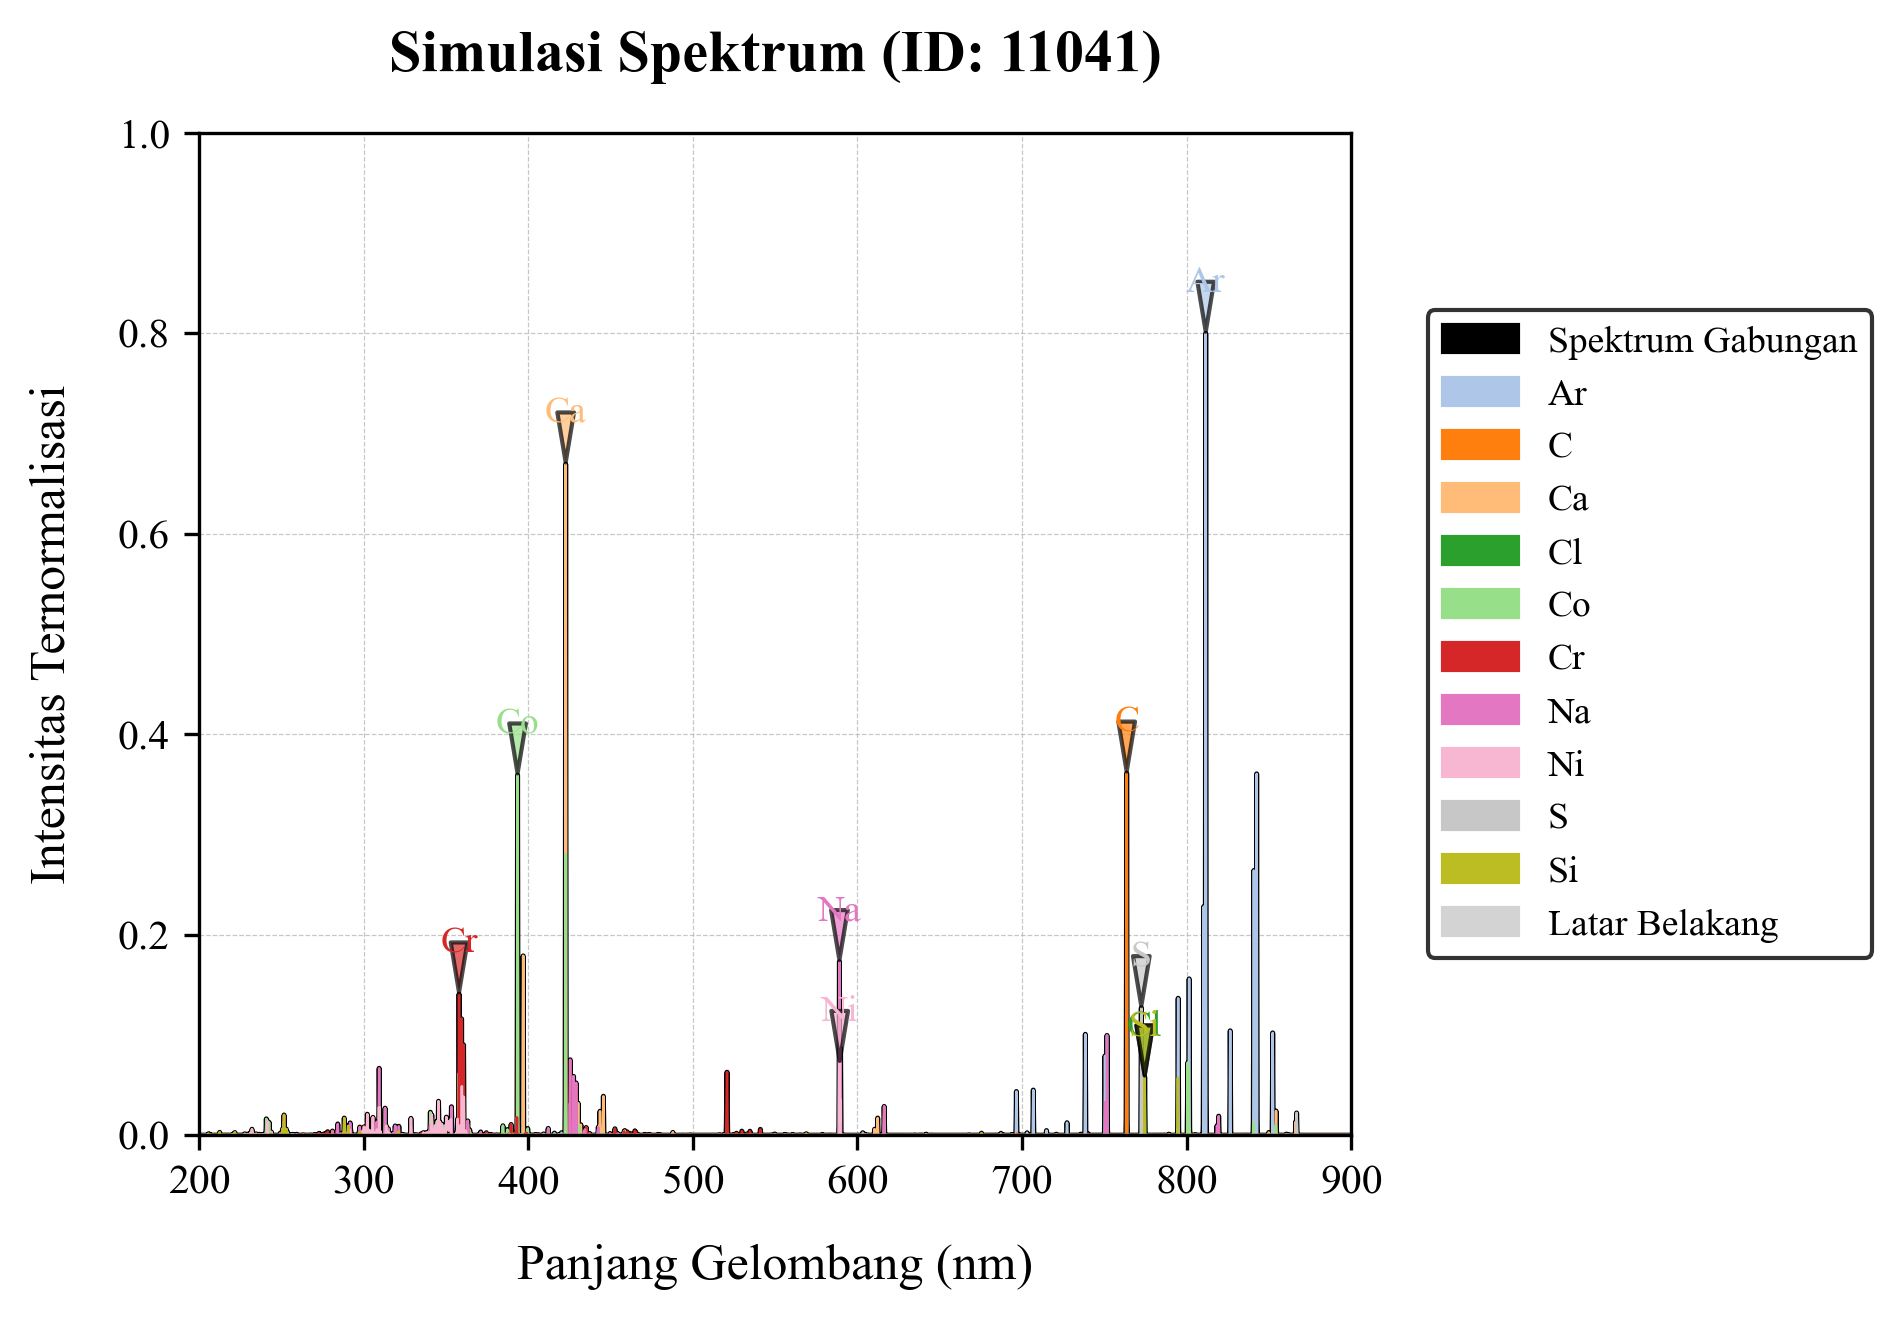
\includegraphics[width=0.9\textwidth]{spectrum_11041.png}
    \caption{Spectral simulation plot for sample 11041.}
    \label{fig:spectrum_11041}
\end{figure}

\clearpage

\section{Sample: 7548}
\subsection{Simulation Parameters}
\begin{table}[h!]
    \centering
    \begin{tabular}{ll}
        \toprule
        \textbf{Parameter} & \textbf{Value} \\
        \midrule
        Temperature ($T$) & 8838 \,\si{K} \\
        Electron Density ($n_e$) & 3.13e+15 \,\si{cm^-3} \\
        \bottomrule
    \end{tabular}
    \caption{Simulation parameters for sample 7548.}
    \label{tab:params_7548}
\end{table}

\subsection{Composition Analysis}
\begin{table}[h!]
    \centering
    \begin{tabular}{lcc}
        \toprule
        \textbf{Element} & \textbf{Initial Composition (\%)} & \textbf{Actual Labeled Position (\%)} \\
        \midrule
        Al & 0.00 & 0.00 \\
        Ar & 0.00 & 0.00 \\
        C & 0.00 & 0.00 \\
        Ca & 20.96 & 3.66 \\
        Cl & 20.48 & 0.76 \\
        Co & 9.75 & 34.28 \\
        Cr & 21.92 & 9.69 \\
        Fe & 0.00 & 0.00 \\
        Mg & 10.79 & 8.47 \\
        Mn & 1.61 & 17.24 \\
        N & 0.00 & 0.00 \\
        Na & 6.62 & 7.86 \\
        Ni & 5.59 & 11.67 \\
        O & 0.00 & 0.00 \\
        S & 1.77 & 4.37 \\
        Si & 0.50 & 5.08 \\
        Ti & 0.00 & 0.00 \\
        background & N/A & 38.28 \\

        \midrule
        \textbf{Total (\%)} & & 141.36 \\
        \bottomrule
    \end{tabular}
    \caption{Composition analysis for sample 7548.}
    \label{tab:comp_7548}
\end{table}

\subsection{Spectral Plot}
\begin{figure}[h!]
    \centering
    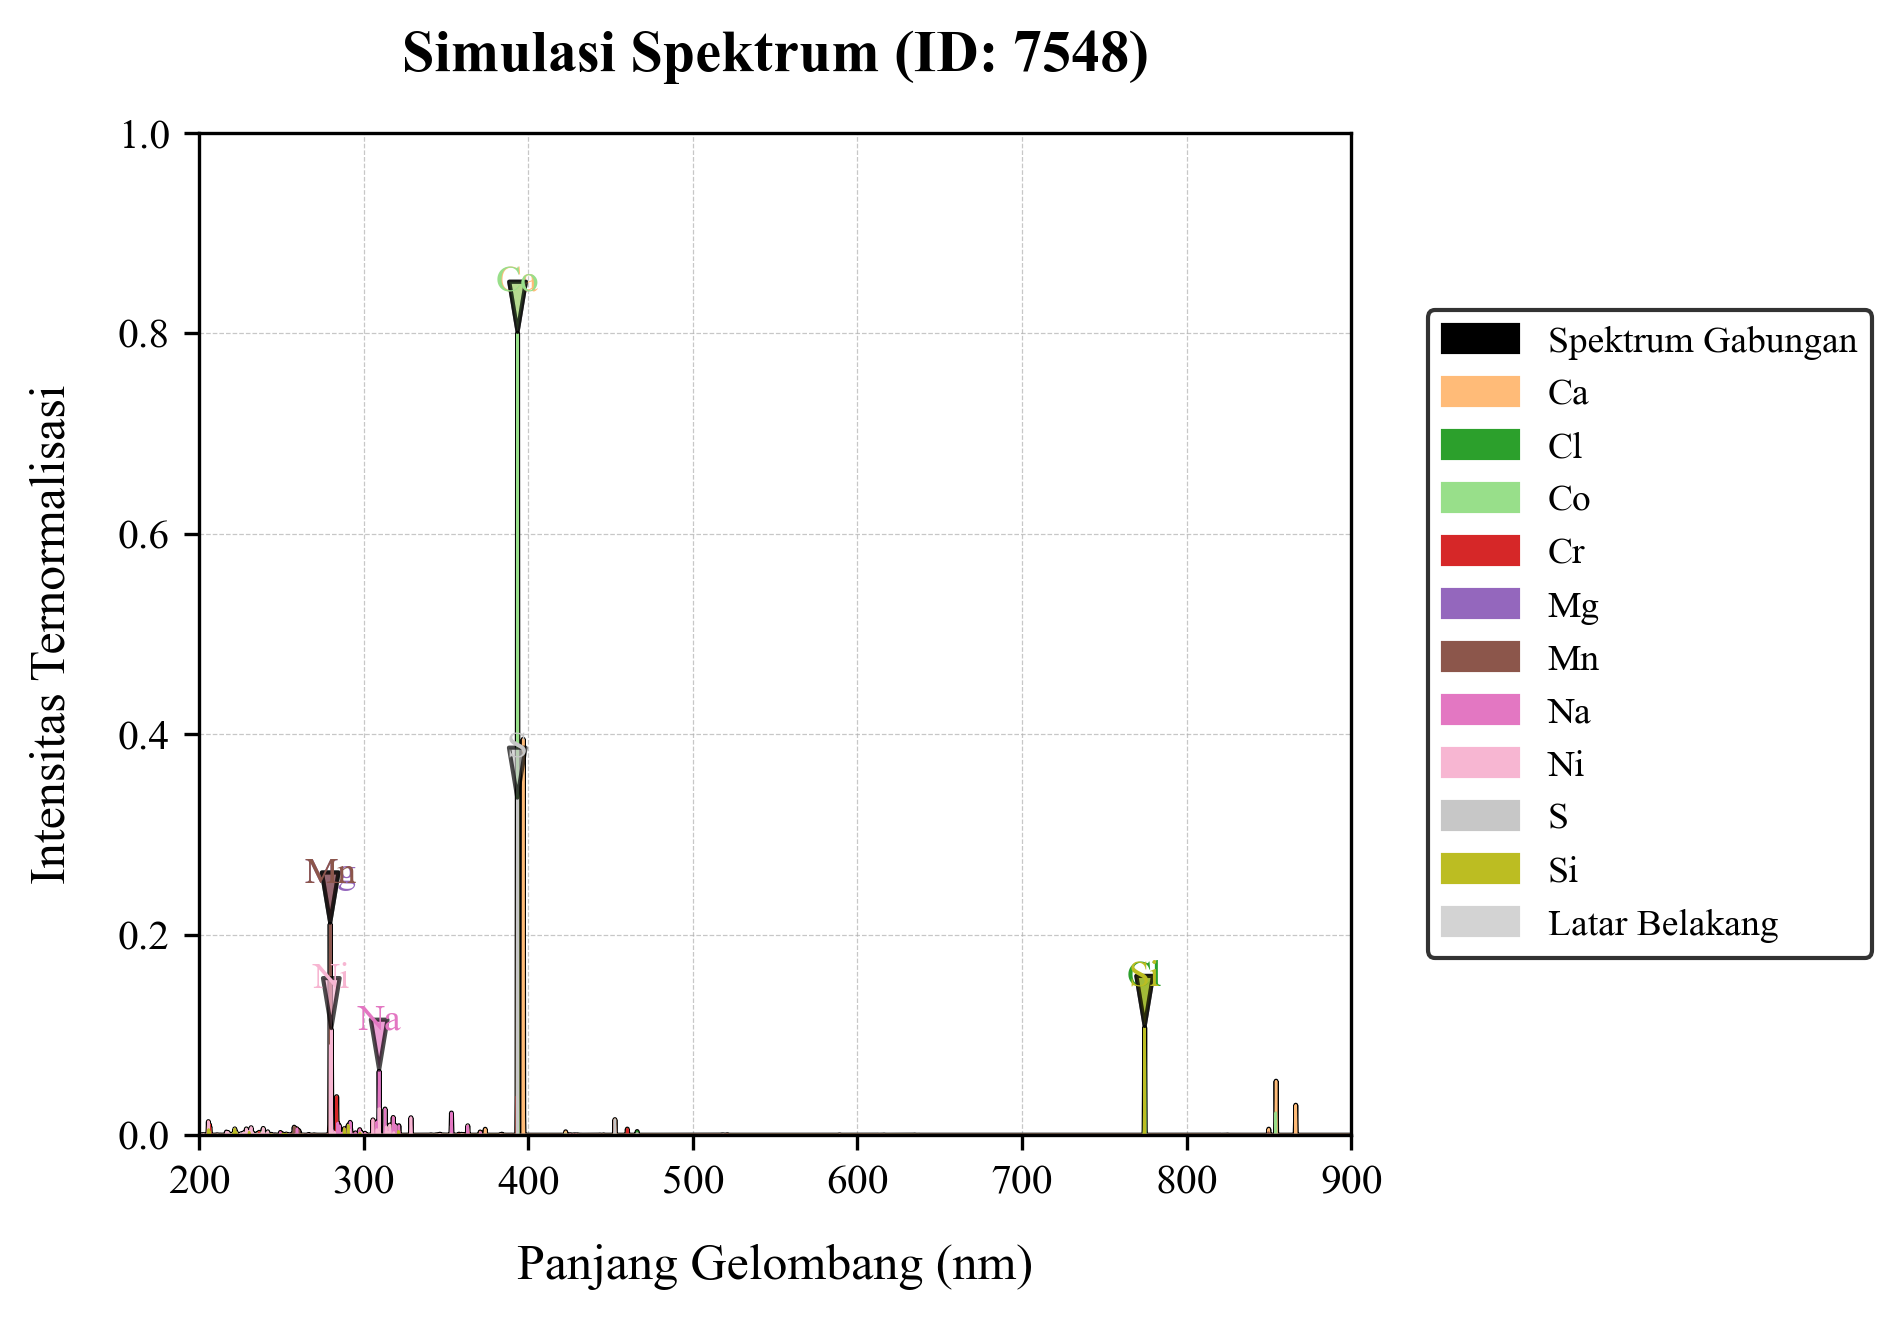
\includegraphics[width=0.9\textwidth]{spectrum_7548.png}
    \caption{Spectral simulation plot for sample 7548.}
    \label{fig:spectrum_7548}
\end{figure}

\clearpage

\section{Sample: 6931}
\subsection{Simulation Parameters}
\begin{table}[h!]
    \centering
    \begin{tabular}{ll}
        \toprule
        \textbf{Parameter} & \textbf{Value} \\
        \midrule
        Temperature ($T$) & 9747 \,\si{K} \\
        Electron Density ($n_e$) & 1.48e+15 \,\si{cm^-3} \\
        \bottomrule
    \end{tabular}
    \caption{Simulation parameters for sample 6931.}
    \label{tab:params_6931}
\end{table}

\subsection{Composition Analysis}
\begin{table}[h!]
    \centering
    \begin{tabular}{lcc}
        \toprule
        \textbf{Element} & \textbf{Initial Composition (\%)} & \textbf{Actual Labeled Position (\%)} \\
        \midrule
        Al & 0.00 & 0.00 \\
        Ar & 0.00 & 0.00 \\
        C & 0.00 & 0.00 \\
        Ca & 12.47 & 3.66 \\
        Cl & 3.08 & 0.81 \\
        Co & 0.00 & 0.00 \\
        Cr & 2.53 & 9.69 \\
        Fe & 0.00 & 0.00 \\
        Mg & 6.70 & 8.47 \\
        Mn & 13.08 & 17.24 \\
        N & 6.12 & 9.79 \\
        Na & 7.47 & 7.86 \\
        Ni & 11.91 & 11.67 \\
        O & 7.55 & 4.47 \\
        S & 10.08 & 5.57 \\
        Si & 10.74 & 5.44 \\
        Ti & 8.26 & 28.96 \\
        background & N/A & 35.42 \\

        \midrule
        \textbf{Total (\%)} & & 149.05 \\
        \bottomrule
    \end{tabular}
    \caption{Composition analysis for sample 6931.}
    \label{tab:comp_6931}
\end{table}

\subsection{Spectral Plot}
\begin{figure}[h!]
    \centering
    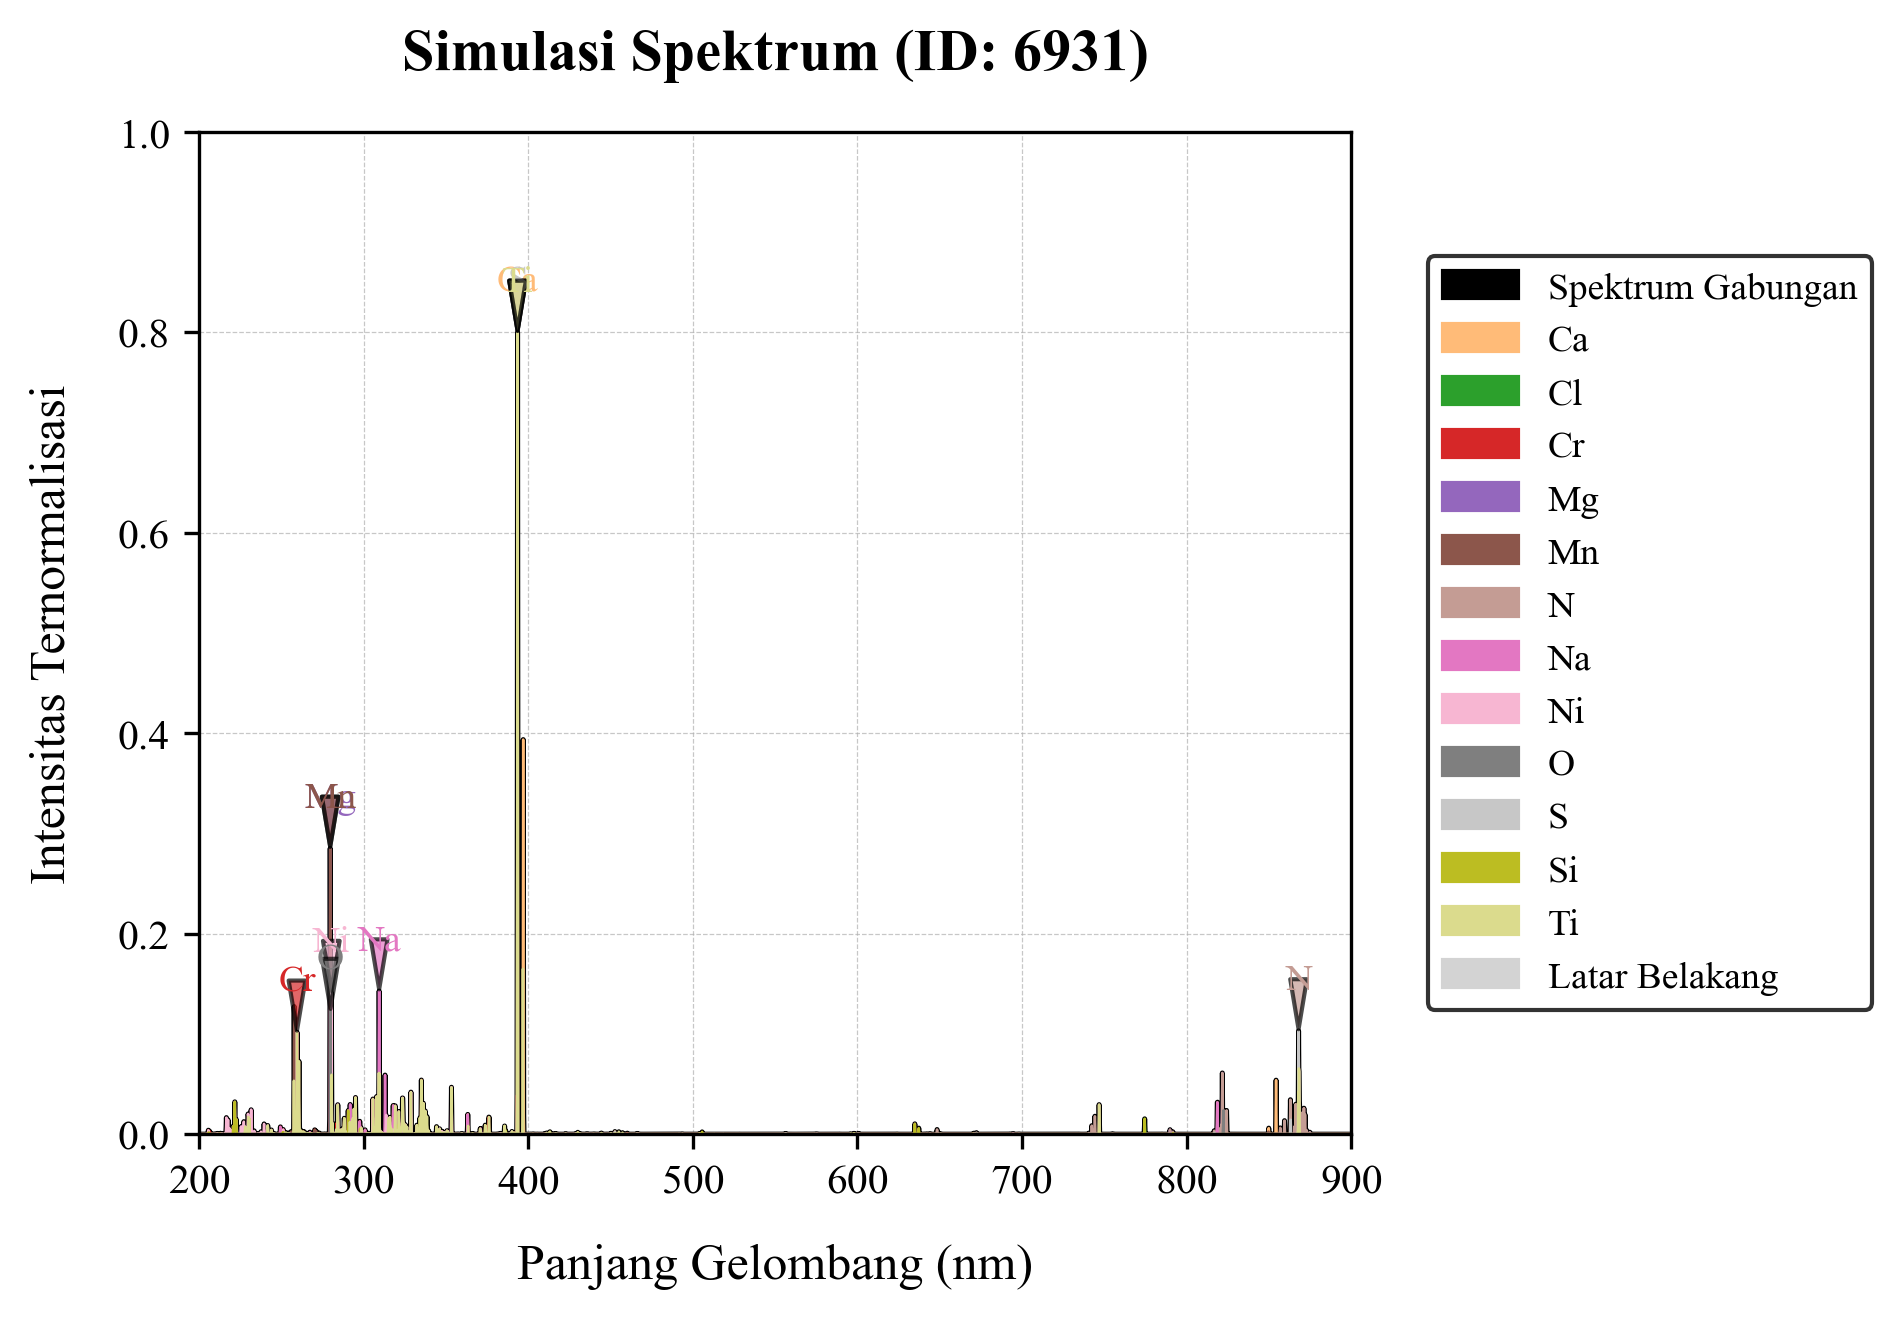
\includegraphics[width=0.9\textwidth]{spectrum_6931.png}
    \caption{Spectral simulation plot for sample 6931.}
    \label{fig:spectrum_6931}
\end{figure}

\clearpage

\section{Sample: 14436}
\subsection{Simulation Parameters}
\begin{table}[h!]
    \centering
    \begin{tabular}{ll}
        \toprule
        \textbf{Parameter} & \textbf{Value} \\
        \midrule
        Temperature ($T$) & 11061 \,\si{K} \\
        Electron Density ($n_e$) & 6.58e+15 \,\si{cm^-3} \\
        \bottomrule
    \end{tabular}
    \caption{Simulation parameters for sample 14436.}
    \label{tab:params_14436}
\end{table}

\subsection{Composition Analysis}
\begin{table}[h!]
    \centering
    \begin{tabular}{lcc}
        \toprule
        \textbf{Element} & \textbf{Initial Composition (\%)} & \textbf{Actual Labeled Position (\%)} \\
        \midrule
        Al & 4.04 & 11.28 \\
        Ar & 10.71 & 17.75 \\
        C & 0.00 & 0.00 \\
        Ca & 9.80 & 3.66 \\
        Cl & 11.62 & 0.85 \\
        Co & 0.00 & 0.00 \\
        Cr & 4.15 & 9.69 \\
        Fe & 0.00 & 0.00 \\
        Mg & 5.31 & 8.59 \\
        Mn & 7.98 & 17.24 \\
        N & 0.77 & 9.89 \\
        Na & 7.19 & 7.86 \\
        Ni & 12.80 & 11.67 \\
        O & 7.07 & 4.79 \\
        S & 13.90 & 5.57 \\
        Si & 4.66 & 5.44 \\
        Ti & 0.00 & 0.00 \\
        background & N/A & 32.08 \\

        \midrule
        \textbf{Total (\%)} & & 146.36 \\
        \bottomrule
    \end{tabular}
    \caption{Composition analysis for sample 14436.}
    \label{tab:comp_14436}
\end{table}

\subsection{Spectral Plot}
\begin{figure}[h!]
    \centering
    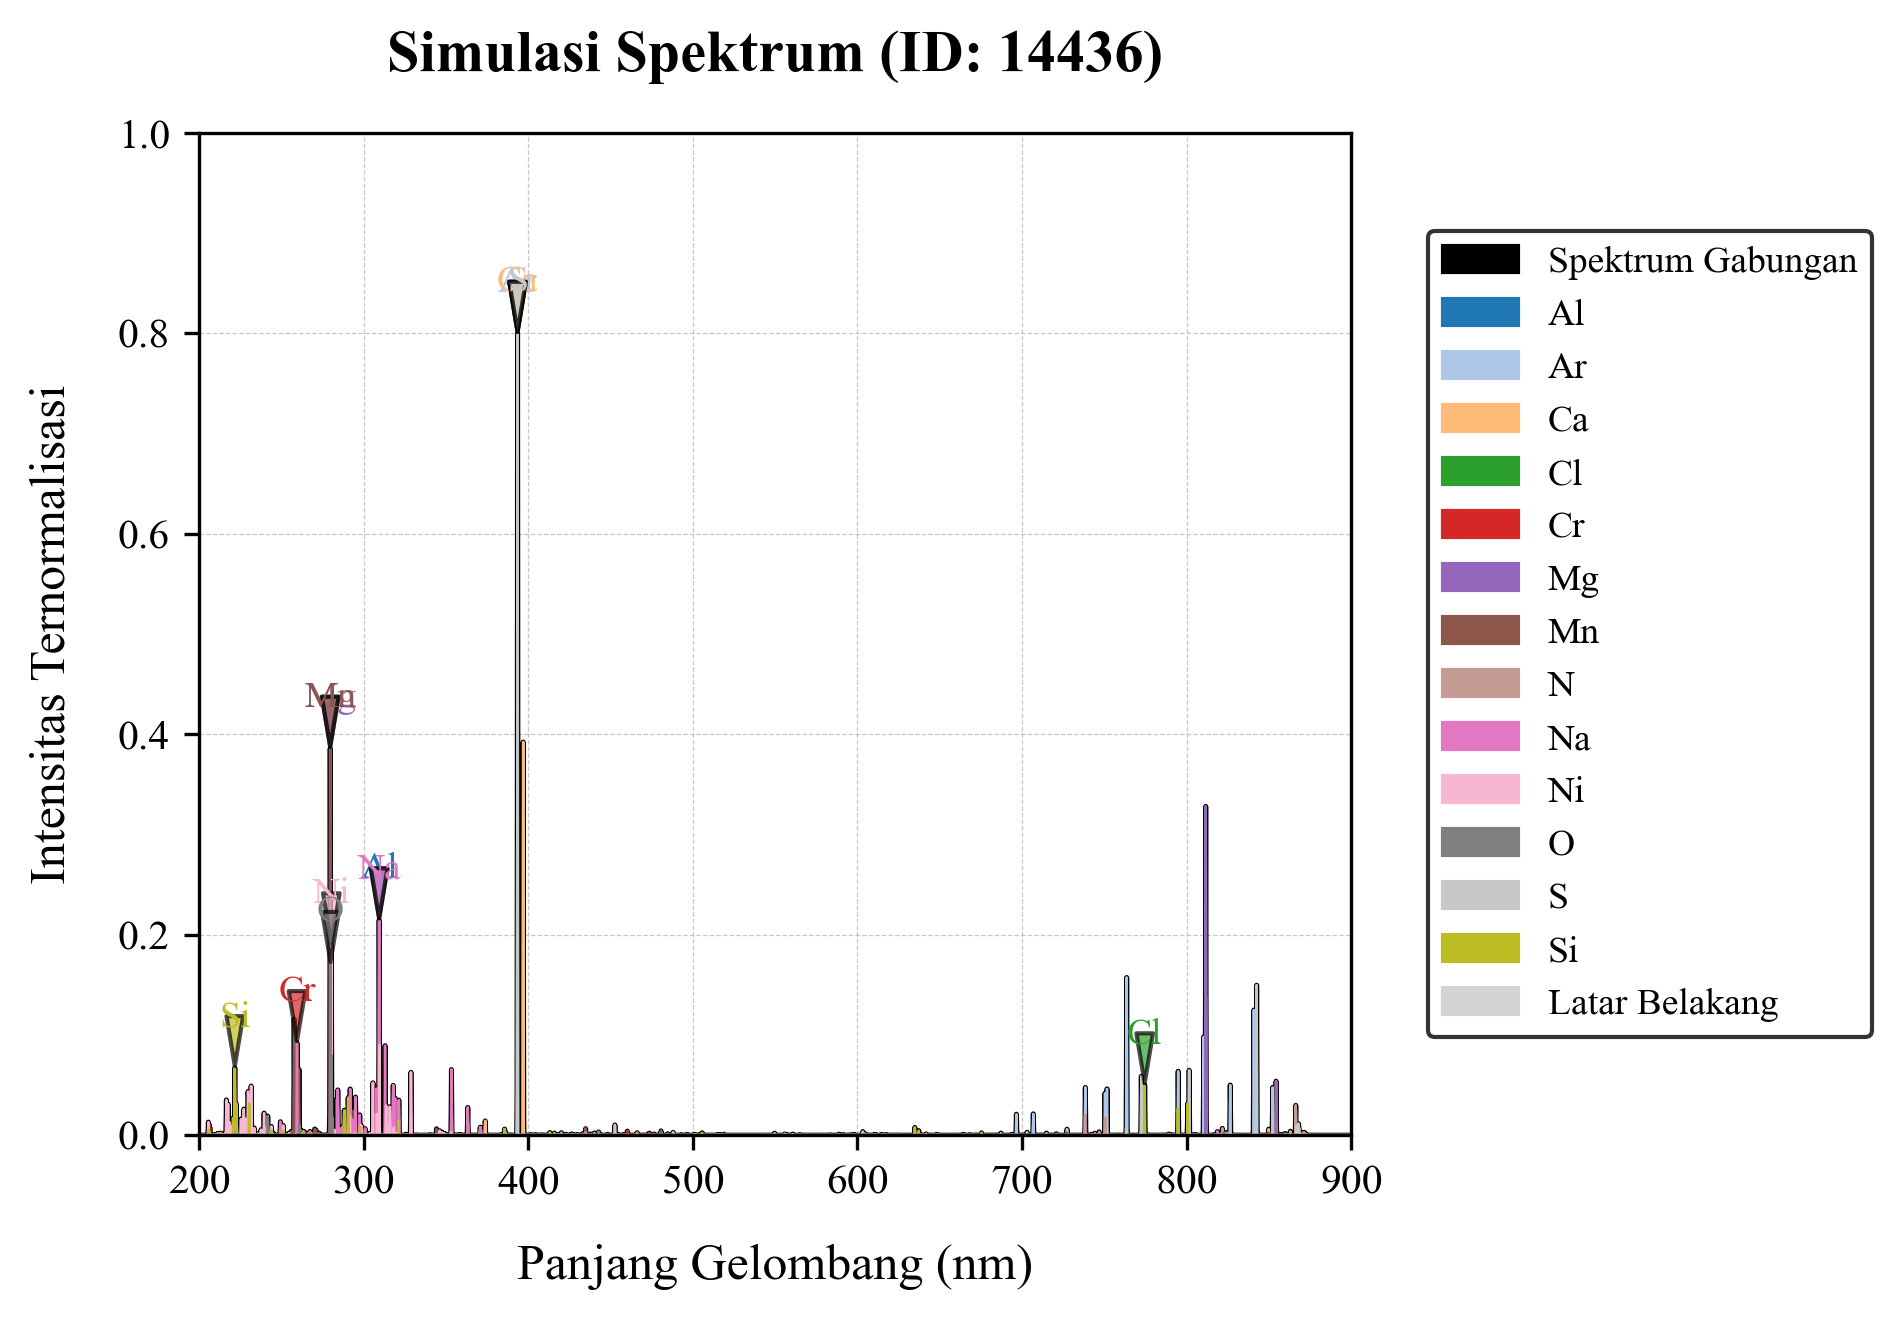
\includegraphics[width=0.9\textwidth]{spectrum_14436.png}
    \caption{Spectral simulation plot for sample 14436.}
    \label{fig:spectrum_14436}
\end{figure}

\clearpage

\section{Sample: 5892}
\subsection{Simulation Parameters}
\begin{table}[h!]
    \centering
    \begin{tabular}{ll}
        \toprule
        \textbf{Parameter} & \textbf{Value} \\
        \midrule
        Temperature ($T$) & 12778 \,\si{K} \\
        Electron Density ($n_e$) & 9.55e+15 \,\si{cm^-3} \\
        \bottomrule
    \end{tabular}
    \caption{Simulation parameters for sample 5892.}
    \label{tab:params_5892}
\end{table}

\subsection{Composition Analysis}
\begin{table}[h!]
    \centering
    \begin{tabular}{lcc}
        \toprule
        \textbf{Element} & \textbf{Initial Composition (\%)} & \textbf{Actual Labeled Position (\%)} \\
        \midrule
        Al & 0.00 & 0.00 \\
        Ar & 0.00 & 0.00 \\
        C & 0.00 & 0.00 \\
        Ca & 1.54 & 3.66 \\
        Cl & 14.47 & 0.85 \\
        Co & 0.00 & 0.00 \\
        Cr & 14.15 & 9.69 \\
        Fe & 7.44 & 67.41 \\
        Mg & 10.37 & 8.64 \\
        Mn & 6.01 & 17.24 \\
        N & 7.83 & 16.14 \\
        Na & 5.92 & 7.86 \\
        Ni & 15.26 & 11.67 \\
        O & 0.00 & 0.00 \\
        S & 7.46 & 5.57 \\
        Si & 9.55 & 5.44 \\
        Ti & 0.00 & 0.00 \\
        background & N/A & 18.92 \\

        \midrule
        \textbf{Total (\%)} & & 173.10 \\
        \bottomrule
    \end{tabular}
    \caption{Composition analysis for sample 5892.}
    \label{tab:comp_5892}
\end{table}

\subsection{Spectral Plot}
\begin{figure}[h!]
    \centering
    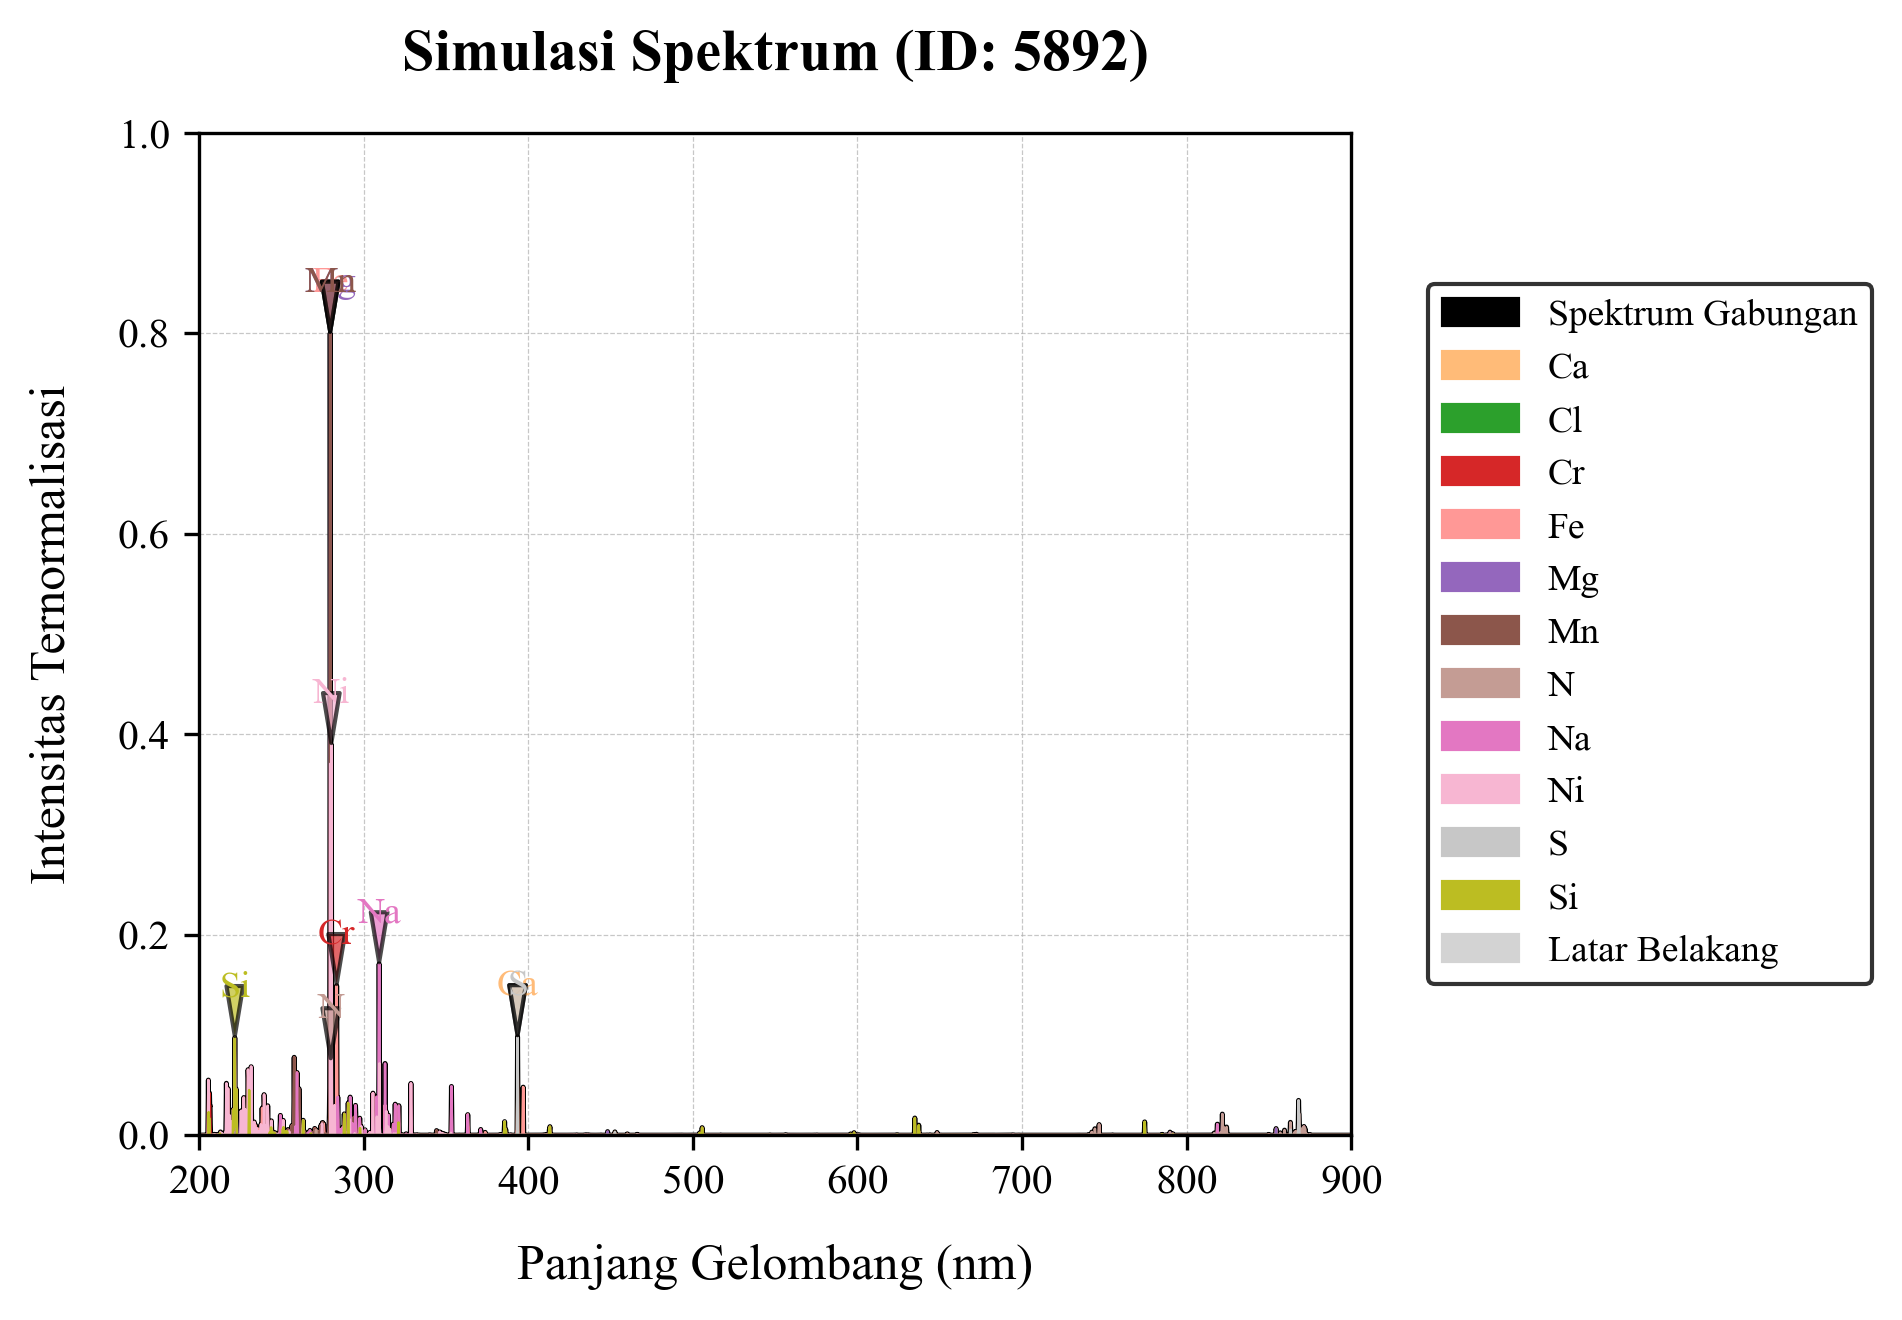
\includegraphics[width=0.9\textwidth]{spectrum_5892.png}
    \caption{Spectral simulation plot for sample 5892.}
    \label{fig:spectrum_5892}
\end{figure}

\clearpage

\end{document}
